
\chapter{Vectors in Three Dimensions}

Fundamentally, vectors are mathematical objects that we can add together and take multiples of, in both cases obtaining another vector. We will consider vectors in a general setting later on, but in this chapter we will consider vectors in $\R^3$, three dimensional space. Specifically, we will take a geometric approach, thinking of vectors as position vectors and using Euclidean notions of points, lines, planes, etc.

We begin by choosing a point $O$ as the origin. Then points $A$ and $B$ have position vectors
$$
\vv{a} = \overrightarrow{OA}, \quad\quad \vv{b} = \overrightarrow{OB}.
$$

\begin{center}
	\begin{tikzpicture}
	\coordinate (origin) at (0,0);
	\coordinate (a) at (4, 0.25);
	\coordinate (b) at (1.5, 2.25);

	\draw (origin) node [anchor=north east] {$O$};

	\draw [->,>=stealth] (origin) -- (a) node [anchor=north west] {$A$} node [pos=0.6, anchor=north] {$\vv{a}$};
	\draw [->,>=stealth] (origin) -- (b) node [anchor=north west] {$B$} node [pos=0.6, anchor=north west] {$\vv{b}$};
	\end{tikzpicture}
\end{center}

The vectors have length $|\vv{a}| = |\overrightarrow{OA}|$, the distance between $O$ and $A$. We also let $\vv{0}$ denote the position vector of $O$.

\section{Vector Addition and Scalar Multiplication}

The most important operations on vectors (in $\R^3$ and in general) is vector addition and scalar multiplication. We define these geometrically as follows.

\begin{definition}[Scalar Multiplication in $\R^3$]
	GIven $\vv{a}$, the position vector for a point $A$, and a scalar $\lambda \in \R$, we define \vocab{scalar multiplication} $\lambda \vv{a}$ to be the position vector for the point $A'$ on the line $OA$ such that
	$$
	|\lambda \vv{a} | = |OA'| = |\lambda| |\vv{a}|,
	$$
	with the vector being in the direction $\overrightarrow{OA}$ if $\lambda$ is positive, and in the opposite direction otherwise.
\end{definition}

\begin{center}
	\begin{tikzpicture}
	\coordinate (origin) at (0,0);
	\coordinate (a) at (2, 0.17);

	\draw (origin) node [anchor=north east] {$O$};

	\draw [->,>=stealth, dashed] ($(origin)  - (a) - (a)$) -- ($(a) + (a) + (a) + (a) $);

	\draw [->,>=stealth, color=blue] (origin) -- ($(a) + (a) + (a)$) node [anchor=north west, color=black] {$A'$} node [pos=0.8, anchor=north] {$\lambda\vv{a}$};
	\draw [->,>=stealth, color=black] (origin) -- ($(a)$) node [anchor=north west, color=black] {$A$} node [pos=0.6, anchor=north, color=black] {$\vv{a}$};
	
	\end{tikzpicture}
\end{center}

If two vectors are scalar multiples of each other, then we say that they are \vocab{parallel}. Specifically, we write $\vv{a} \parallel \vv{b}$ if and only if $\vv{a} = \lambda \vv{b}$ or $\vv{b} = \lambda \vv{a}$ for some $\lambda \in \R$. Notably, $\vv{a} \parallel \vv{0}$ for all vectors $\vv{a}$.


\begin{definition}[Vector Addition in $\R^3$]
	Given $\vv{a}$ and $\vv{b}$, position vectors of points $A$ and $B$, if $\vv{a} \not \parallel \vv{b}$, we construct the parallelogram $OACB$, and define \vocab{vector addition} $\vv{a} + \vv{b} = \vv{c}$. 
\end{definition}


\begin{center}
	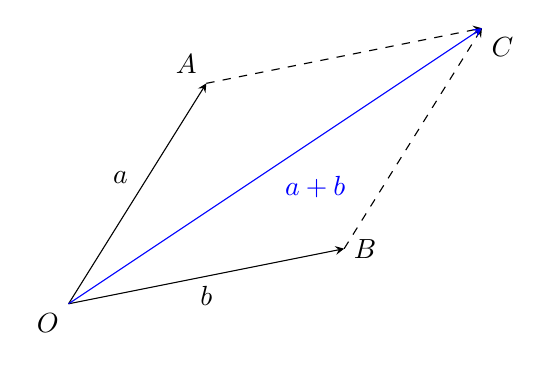
\begin{tikzpicture}[xscale=1.4, yscale=1.4]
	\draw (0, 0) node [anchor=north east] {$O$};
	\draw [->,>=stealth] (0, 0) -- (2.5, 0.5) node [anchor=west] {$B$} node [pos=0.5, anchor=north] {$\vv{b}$};
	\draw [->,>=stealth] (0, 0) -- (1.25, 2.0) node [anchor=south east] {$A$} node [pos=0.5, anchor=south east] {$\vv{a}$};
	\draw [->,>=stealth, dashed] (1.25, 2.0) -- (3.75, 2.5);
	\draw [->,>=stealth, dashed] (2.5, 0.5) -- (3.75, 2.5);
	\draw [->,>=stealth, color=blue] (0,0) -- (3.75, 2.5) node [pos=0.5, anchor=north west] {$\vv{a} + \vv{b}$};
	\draw (3.75, 2.5) node [anchor=north west] {$C$};
	\end{tikzpicture}
  \end{center}

If $\vv{a} \parallel \vv{b}$, then writing $\vv{a} = \alpha \vv{u}$ and $\vv{b} = \beta \vv{u}$ where $\vv{u}$ is a unit vector, then $\vv{a} + \vv{b} = (\alpha+ \beta) \vv{u}$.

Given some set of vectors $\vv{v_1}$, $\vv{v_2}$, $\dots$, $\vv{v_k}$, we can form a \vocab{linear combination}
$$
\lambda_1 \vv{v_1} + \lambda_2 \vv{v_2}  + \cdots + \lambda_k \vv{v_k},
$$
where $\lambda_i \in \R$. With this in mind, we can consider the set of all vectors that can be formed as a linear combination of some vectors.

\begin{definition}[Span]
	For vectors $\vv{v_1}$, $\vv{v_2}$, $\dots$, $\vv{v_k}$, we define their \vocab{span} to be the set
	$$
	\vecspan\{\vv{v_1}, \vv{v_2}, \dots, \vv{v_k} \} = \{ \lambda_1 \vv{v_1} + \lambda_2 \vv{v_2}  + \cdots + \lambda_k \vv{v_k} \mid \lambda_i \in \R \}.
	$$
\end{definition}

If two vectors $\vv{a} \not \parallel \vv{b}$, then $\vecspan\{\vv{a}, \vv{b}\}$ is a plane through $OAB$.

Vector addition and scalar multiplication obey some basic properties that you should keep in mind, as they will be used again when we define vectors in a general sense.

\begin{proposition}[Basic Properties of Vector Operations]
For any vectors $\vv{a}$, $\vv{b}$ and $\vv{c}$,
\begin{enumerate}[label=(\roman*)]
	\item Vectors along with vector addition form an abelian group.
	\item $\lambda(\vv{a} + \vv{b}) = \lambda \vv{a} + \lambda \vv{b}$.
	\item $(\lambda + \mu)\vv{a} = \lambda\vv{a} + \mu\vv{a}$.
	\item $\lambda(\mu \vv{a}) = (\lambda \mu) \vv{a}$.
\end{enumerate}
\end{proposition}
\begin{proof}[Proof Sketch]
	Check geometric definitions. Checking associativity of vector addition will require the construction of a parallelepiped.
\end{proof}


\section{The Dot Product}

We saw in the previous section how to add vectors, and how to multiply a vector by a scalar. In the next two sections, we will consider how to multiply a vector and a vector. 
We will first define the \emph{scalar} or \emph{dot product}.
Consider two vectors $\vv{a}$ and $\vv{b}$, with the angle between then being $\theta$ as shown.

\begin{center}
    \begin{tikzpicture}
        \coordinate (origin) at (0,0);
        \coordinate (z) at (1.75, 1.9);
        \coordinate (z1) at (3.25, 0);

        % \draw (0, 0) node [anchor=north east] {$O$};
        \draw [->,>=stealth] (0, 0) -- (z1) node [anchor=west] {$\vv{a}$};
        %  node [pos=0.5, anchor=north] {$\vv{a}$};
        \draw [->,>=stealth] (0, 0) -- (z) node [anchor=west] {$\vv{b}$};
        %  node [pos=0.5, anchor=south east] {$\vv{b}$};
        \pic [draw, ->, angle eccentricity=1.2, angle radius=1.25cm, color=purple] {angle = z1--origin--z};
        \draw (0.8, 0.38) node {$\theta$};
	\end{tikzpicture}
  \end{center}

\begin{definition}[Dot Product]
    For two vectors $\vv{a}$ and $\vv{b}$, and $\theta$ the angle between them as shown, we define the \vocab{scalar} or \vocab{dot product} as
    $$
    \vv{a} \cdot \vv{b} = |\vv{a}| |\vv{b}| \cos \theta.
    $$

    [Note that $\theta$ is defined unless $\vv{a}$ or $\vv{b}$ is zero, but then $|\vv{a}| = 0$ or $|\vv{b}| = 0$ and $\vv{a} \cdot \vv{b} = 0$.]
\end{definition}

The scalar product encodes an angle condition, and gives us a dot for perpendicularity. We say vectors $\vv{a}$ and $\vv{b}$ are \vocab{orthogonal} or \vocab{perpendicular} if and only if $\vv{a} \cdot \vv{b} = 0$. This corresponds with $\theta = \pm \pi/2$, or with either $|\vv{a}| = 0$ or $|\vv{b}| = 0$.

There is a geometric interpretation of the dot product. Fundamentally, the dot product is a \emph{projection}. For $\vv{a} \neq \vv{0}$, the quantity $|\vv{b}| \cos \theta$ is the component of $\vv{b}$ when projected along the direction of $\vv{a}$.

\begin{center}
    \begin{tikzpicture}
        \coordinate (origin) at (0,0);
        \coordinate (z) at (1.75, 1.9);
        \coordinate (z1) at (3.25, 0);

        \draw [dashed] (0, 0) -- (5.25, 0);

        \draw [color=blue, dashed] (z) -- (1.75, 0);

        \fill (1.75,0)  circle[color=blue, radius=1pt];

        % \draw (0, 0) node [anchor=north east] {$O$};
        \draw [->,>=stealth] (0, 0) -- (z1) node [anchor=north] {$\vv{a}$};
        %  node [pos=0.5, anchor=north] {$\vv{a}$};
        \draw [->,>=stealth] (0, 0) -- (z) node [anchor=west] {$\vv{b}$};
        %  node [pos=0.5, anchor=south east] {$\vv{b}$};
        \pic [draw, ->, angle eccentricity=1.2, angle radius=0.8cm, color=purple] {angle = z1--origin--z};
        \draw (0.533333333, 0.253333333) node {\small $\theta$};

        % \draw (1.75, 0) node [anchor=north] {$\vv{b}_{\parallel}$};
        \draw [color=blue] (0,0) -- (1.75, 0);

        \draw [decoration={brace, mirror, raise=0.4cm}, decorate] (0,0) -- (1.75, 0) node [pos=0.5, anchor=north, yshift=-0.45cm] {\footnotesize $|\vv{b}| \cos \theta$};
        \draw [densely dashed] (0,0) -- (0, -0.4cm);
        \draw [densely dashed] (1.75,0) -- (1.75, -0.4cm);
	\end{tikzpicture}
  \end{center}

  \begin{proposition}[Basic Properties of the Dot Product]
      For any vectors $\vv{a}$ and $\vv{b}$,
      \begin{enumerate}[label=(\roman*)]
          \item $\vv{a} \cdot \vv{b} = \vv{b} \cdot \vv{a}$.
          \item $\vv{a} \cdot \vv{a} = |a|^2 \geq$, and $\vv{a} \cdot \vv{a} = 0$ if and only if $\vv{a} = \vv{0}$.
          \item $(\lambda \vv{a}) \cdot \vv{b} = \lambda (\vv{a} \cdot \vv{b}) = \vv{a} \cdot (\lambda \vv{b})$.
          \item $\vv{a} \cdot (\vv{b} + \vv{c}) = \vv{a} \cdot \vv{b} + \vv{a} \cdot \vv{c}$. 
      \end{enumerate}
  \end{proposition}
  \begin{proof}
      Properties (i) to (iii) follow directly from the definition of the dot product. Property (iv) follows from the geometric interpretation of the dot product shown above. 
  \end{proof}



\section{The Cross Product}

The next operation only works with vectors in three dimensions, and is the \emph{vector} or \emph{cross product}. As before, consider two vectors $\vv{a}$ and $\vv{b}$, and let $\theta$ be measured as shown with respect to $\hat{\vv{n}}$, a unit normal to the plane spanned by $\vv{a}$ and $\vv{b}$.

\begin{center}
    \begin{tikzpicture}
        \coordinate (origin) at (0,0);
        \coordinate (z) at (2.5, 0.6);
        \coordinate (z1) at (3.25, -0.35);

        % \draw (0, 0) node [anchor=north east] {$O$};
        \draw [->,>=stealth] (0, 0) -- (z1) node [anchor=west] {$\vv{a}$};
        %  node [pos=0.5, anchor=north] {$\vv{a}$};
        \draw [->,>=stealth] (0, 0) -- (z) node [anchor=west] {$\vv{b}$};
        %  node [pos=0.5, anchor=south east] {$\vv{b}$};
        \pic [draw, ->, angle eccentricity=1.8, angle radius=1.45cm, color=purple] {angle = z1--origin--z};
        
        \draw (1, 0.08) node {$\theta$};

        \draw [->,>=stealth, color=blue] (0,0) -- (0, 1.5) node [anchor=south] {$\hat{\vv{n}}$};
	\end{tikzpicture}
  \end{center}

  \begin{definition}[Cross Product]
For two vectors $\vv{a}$ and $\vv{b}$ with angle  $\theta$ measured as shown, we define the \vocab{vector} or \vocab{cross product} as
$$
\vv{a} \times \vv{b} = | \vv{a}| |\vv{b}| \sin \theta \hat{\vv{n}},
$$
where $\hat{\vv{n}}$ is a unit vector perpendicular to the plane spanned by $\vv{a}$ and $\vv{b}$.

[$\hat{\vv{n}}$ is defined up to a sign if $\vv{a} \not \parallel \vv{b}$, but changing the sign changes $\theta$ to $2\pi - \theta$, and thus leaves $\vv{a} \times \vv{b}$ unchanged. When $\hat{\vv{n}}$ is not defined ($\vv{a} \parallel \vv{b}$ or $\theta$ not defined), $\vv{a} \times \vv{b} = \vv{0}$.] 
  \end{definition}

  The geometric interpretation of the cross product is that $|\vv{a} \times \vv{b}|$ is the area of the parallelogram as shown.

  \begin{center}
    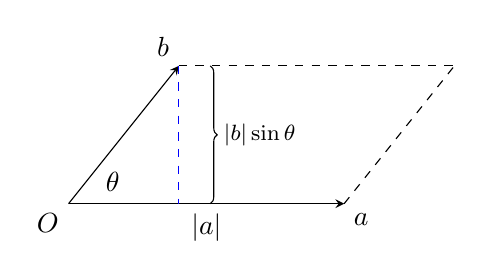
\begin{tikzpicture}[xscale=1.4, yscale=1.4]
    \draw (0, 0) node [anchor=north east] {$O$};
    
    \draw [->,>=stealth] (0, 0) -- (2.5, 0) node [anchor=north west] {$\vv{a}$} node [pos=0.5, anchor=north] {$|\vv{a}|$};
    \draw [->,>=stealth] (0, 0) -- (1, 1.25) node [anchor=south east] {$\vv{b}$};

    \draw (0.4, 0.2) node {$\theta$};

    \draw [dashed] (1, 1.25) -- (3.5, 1.25);
    \draw [dashed] (2.5, 0) -- (3.5, 1.25);

    \draw [dashed, color=blue] (1,1.25) -- (1, 0);
    \draw [decoration={brace, raise=0.4cm}, decorate] (1, 1.25) -- (1, 0) node [pos=0.5, anchor=west, xshift=0.45cm] {\footnotesize $|\vv{b}| \sin \theta$};
    
	% \draw [->,>=stealth, dashed] (1.25, 2.0) -- (3.75, 2.5);
	% \draw [->,>=stealth, dashed] (2.5, 0.5) -- (3.75, 2.5);
	% \draw [->,>=stealth, color=blue] (0,0) -- (3.75, 2.5) node [pos=0.5, anchor=north west] {$\vv{a} + \vv{b}$};
	% \draw (3.75, 2.5) node [anchor=north west] {$C$};
    \end{tikzpicture}
  \end{center}

  The direction of $\vv{a} \times \vv{b}$ gives the orientation of this parallelogram in space.   

For an alternate geometric interpretation, fix a vector $\vv{a}$ and consider some vector $\vv{x}$ with $\vv{x} \perp \vv{a}$. Then the transformation $\vv{x} \longmapsto \vv{a} \times \vv{x}$ corresponds with scaling $\vv{x}$ by $\vv{a}$ and rotating by $\pi/2$ in the plane perpendicular to $\vv{a}$.

\begin{proposition}[Basic Properties of the Cross Product]
    For vectors $\vv{a}$, $\vv{b}$ and $\vv{c}$,
    \begin{enumerate}[label=(\roman*)]
        \item $\vv{a} \times \vv{b} = - (\vv{b} \times \vv{a})$.
        \item $(\lambda \vv{a}) \times \vv{b} = \lambda (\vv{a}) \times \vv{b})$.
        \item $\vv{a} \times (\vv{b} + \vv{c}) = \vv{a} \times \vv{b} + \vv{a} \times \vv{c}$.
        \item $\vv{a} \times \vv{b} = \vv{0}$ if and only if $\vv{a} \perp \vv{b}$.
        \item $\vv{a} \times \vv{b} \perp \vv{a}, \vv{b}$, so $\vv{a} \cdot (\vv{a} \times \vv{b}) = \vv{b} \cdot (\vv{a} \times \vv{b}) = 0$. 
    \end{enumerate}
\end{proposition}
\begin{proof}[Proof Sketch]
    Check definitions.
\end{proof}

\section{Orthonormal Bases and Components}

So far we have considered vectors in a purely geometric sense. But just as a coordinate system can be used to reason about geometry, basis (and by extension components) can be used to reason about vectors. We will look at bases again in a more general setting later on, but for now we will focus on vectors in three dimensions.

When we use a cartesian coordinate system, we pick a set of axes and using them, we can describe the position of any point. In a similar way, a \emph{basis} is a set of vectors that span the space. That is, any vector can be written as a linear combination of vectors in the set. However we also have an additional requirement: this linear combination must be unique.

\begin{definition}[Basis -- Informal]
    We say that a set of vectors is a \vocab{basis} if any vector can be uniquely written as a linear combination of vectors in the set.
\end{definition}

Before we continue, it's helpful when working with vectors in three dimensions (and in other settings) to pick basis vectors in a certain way. We introduce the following definition.

\begin{definition}[Orthonormal]
    We say that a set of vectors $\{\vv{v_1}, \vv{v_2}, \dots, \vv{v_n} \}$ is \vocab{orthonormal} if they are all unit vectors and are orthogonal to each other. That is, if $|\vv{v_i}| = 1$ and
    $$
        \vv{v_i} \cdot \vv{v_j} = \begin{cases}
            1 &\mbox{if } i = j, \\
            0 &\mbox{if } i \neq j.
           \end{cases}
    $$
    for all $1 \leq i, j \leq n$.
\end{definition}

Now choose vectors $\vv{e}_1, \vv{e}_2, \vv{e}_3$ that are \vocab{orthonormal}. Then the set $\{\vv{e}_i \}$ is a basis, so for any vector $\vv{a}$, we can write
$$
\vv{a} = \sum_{i} a_i \vv{e}_i = a_1 \vv{e}_1 + a_2 \vv{e}_2 + a_3 \vv{e}_3,
$$
and each coefficient is uniquely defined by $a_i = \vv{e}_i \cdot \vv{a}$. Note that this only works because of our orthonormal condition.

Recalling that dot products correspond to projections, we can see that this really is analogous to a cartesian coordinate system.

\begin{center}
    \begin{tikzpicture}
        \draw [->,>=stealth] (0, 0) -- (0, 2) node [anchor=south] {$\vv{e}_3$};
        \draw [->,>=stealth] (0, 0) -- (1.95, -0.4) node [anchor=west] {$\vv{e}_2$};
        \draw [->,>=stealth] (0, 0) -- (-1.45, -1) node [anchor=north east] {$\vv{e}_1$};

        \draw [dashed, color=blue] (0.85, 1.6) -- (0, 1.675);

        \draw [->,>=stealth, color=red] (0, 0) -- (0.85, 1.6) node [anchor=south west] {$\vv{a}$};

        \draw [decoration={brace, raise=0.25cm}, decorate, color=blue] (0,0) -- (0, 1.675) node [pos=0.5, anchor=east, xshift=-0.3cm] {\footnotesize $a_3$}; 
    \end{tikzpicture}
\end{center}
Once we have specified the basis vectors $\{\vv{e}_i\}$, we can then identify the vector $\vv{a}$ by its \vocab{components}, writing 
$$
\vv{a} = (a_1, a_2, a_3), \quad \quad \text{or} \quad \quad \vv{a} = \begin{pmatrix} a_1 \\ a_2 \\ a_3 \end{pmatrix},
$$
which is a \vocab{row} or \vocab{column} vector respectively\footnote{The difference will be important when we move onto matrices.}.

An advantage of writing vectors in this form is that we can work directly with the components.

\subsection{Dot Product in Components}

For two vectors $\vv{a} = (a_1, a_2, a_3)$ and $\vv{b} = (b_1, b_2, b_3)$, their dot product is
$$
\vv{a} \cdot \vv{b} = (a_1, a_2, a_3) \cdot (b_1, b_2, b_3) = a_1 b_1 + a_2 b_2 + a_3 b_3.
$$

We can use this to directly calculate the length of the vector,
with
$$
\vv{a}\cdot\vv{a} = |\vv{a}|^2 = a_1 ^2 + a_2 ^2 + a_3^2.
$$


